% !TeX spellcheck = russian-aot

\newcommand{\pictureone}{
	\begin{figure}[!htbp]
		\fontsize{10}{12}
		\centering
		\begin{tikzpicture}[thick, on grid]
			% Server
			\node [block] (server) {Сервер};
			% Database
			\node [block, right= of server] (bd) {База данных};
			\draw[<->] (server) -- node[link, above] {Данные о растениях} (bd); 
			% Receiver API
			\node [block, below left= of server] (ext-api) {API для получения опубликованных данных};
			\draw[->] (server) -- node[link, below right] {Обработанные данные} (ext-api);
			
			% Service site
			\node [block, above= of server] (service-site) {Сервисный сайт};
			\draw[<->] (server) -- node[link, right] {Модерация и изменение статуса данных} (service-site);
			% Public site
			\node [block, above left= of server] (public-site) {Сайт с опубликованными данными};
			\draw[->] (ext-api) -- node[link, right] {Запрошенные пользователем данные} (public-site);
			
			% Sender API
			\node [block, below right= of server] (int-api) {API для получения данных};
			\draw[<-] (server) -- node[link, below left] {Данные, полученные от пользователей} (int-api);
			% WEB client
			\node [block, below= of ext-api] (web-cli) {WEB клиент};
			\draw[<-] (int-api) to[bend left=35, looseness=1.8] node[link, below right] {Данные о найденном растении} (web-cli);
			\draw[->] (ext-api) -- node[link, left] {Cортированные данные} (web-cli);
			% Android client
			\node [block, right= of web-cli] (and-cli) {Android клиент};
			\draw[<-] (int-api) -- node[link, above left] {Данные о найденном растении} (and-cli);
			\draw[->] (ext-api) -- node[link, above right] {Запрошенные пользователем данные} (and-cli);
			% iOS client
			\node [block, right= of and-cli] (ios-cli) {iOS клиент};
			\draw[<-] (int-api) -- node[link, right] {Данные о найденном растении} (ios-cli);
			\draw[->] (ext-api) to[bend right=35, looseness=1.8] node[link, below left] {Запрошенные пользователем данные} (ios-cli);
		\end{tikzpicture}
		\caption{Схема архитектуры}
	\end{figure}
}

\newcommand{\picturetwo}{
	\begin{figure}[!htbp]
		\fontsize{10}{12}
		\centering
		\begin{tikzpicture}[thick, node distance = 7cm and 9cm, on grid]
			% User
			\node [block, text width=7.5cm, align=left] (user) {
				\centering{\textbf{Пользователь}}
				\begin{itemize}[parsep=0pt, leftmargin=*, labelindent=0cm]
					\item \under{Номер пользователя}
					\item Хэш сумма пароля
					\item Имя
					\item Дата регистрации в системе
					\item Время последнего входа в систему
					\item Является ли пользователь администратором
					\item Является ли пользователь специалистом
					\item Активен ли аккаунт пользователя
					\item Фото профиля
					\item Уменьшенное фото профиля
				\end{itemize}
			};
			% Report
			\node [block, text width=4.5cm, align=left, right= of user] (report) {
				\centering{\textbf{Отчёт}}
				\begin{itemize}[parsep=0pt, leftmargin=*, labelindent=0cm]
					\item \under{Номер отчёта}
					\item Дата и время наблюдения
					\item Адрес
					\item Первый комментарий
					\item Координаты
					\item Статус
					\item Вид растения
					\item Фотографии
				\end{itemize}
			};
			\draw[-<, dashed] (user) -- (report);
			% Photo
			\node [block, text width=4cm, align=left, below right= of user] (photo) {
				\centering{\textbf{Фотография}}
				\begin{itemize}[parsep=0pt, leftmargin=*, labelindent=0cm]
					\item \under{Номер фотографии}
					\item Фотография
					\item Уменьшенная фотография
				\end{itemize}
			};
			\draw[-, dashed] (report) -- ($(report)!0.6!(photo)$);
			\draw[-<] ($(report)!0.6!(photo)$) -- (photo);
			% Comment
			\node [block, text width=4cm, align=left, below= of user] (comment) {
				\centering{\textbf{Комментарий}}
				\begin{itemize}[parsep=0pt, leftmargin=*, labelindent=0cm]
					\item \under{Номер комментария}
					\item Текст комментария
				\end{itemize}
			};
			\draw[-<, dashed] (user) -- (comment);
			\draw[-, dashed] (report) -- ($(report)!0.6!(comment)$);
			\draw[-<] ($(report)!0.6!(comment)$) -- (comment);
		\end{tikzpicture}
		\caption{ER диаграмма модели}
	\end{figure}
}

\newcommand{\picturethree}{
	\begin{figure}[!htbp]
		\fontsize{10}{12}
		\centering
		\begin{tikzpicture}[thick, node distance = 0.75cm, on grid]
			% User
			\node[inner, text width=7cm, label={[name=user]Пользователь}] (inner_user0) {\under{Номер пользователя}};
			\node[inner, text width=7cm, below= of inner_user0] (inner_user1) {Адрес электронной почты};
			\node[inner, text width=7cm, below= of inner_user1] (inner_user2) {Хэш сумма пароля};
			\node[inner, text width=7cm, below= of inner_user2] (inner_user3) {Имя};
			\node[inner, text width=7cm, below= of inner_user3] (inner_user4) {Дата регистрации в системе};
			\node[inner, text width=7cm, below= of inner_user4] (inner_user5) {Время последнего входа в систему};
			\node[inner, text width=7cm, below= of inner_user5] (inner_user6) {Является ли пользователь администратором};
			\node[inner, text width=7cm, below= of inner_user6] (inner_user7) {Является ли пользователь специалистом};
			\node[inner, text width=7cm, below= of inner_user7] (inner_user8) {Активен ли аккаунт пользователя};
			\node[inner, text width=7cm, below= of inner_user8] (inner_user9) {Фото профиля};
			\node[inner, text width=7cm, below= of inner_user9] (inner_user10) {Уменьшенное фото профиля};
			% Report
			\node[right=7.5cm of inner_user0, inner, label={[name=report]Отчёт}] (inner_report0) {\under{Номер отчёта}};
			\node[inner, below= of inner_report0] (inner_report1) {Номер пользователя};
			\node[inner, below= of inner_report1] (inner_report2) {Дата и время наблюдения};
			\node[inner, below= of inner_report2] (inner_report3) {Адрес};
			\node[inner, below= of inner_report3] (inner_report4) {Первый комментарий};
			\node[inner, below= of inner_report4] (inner_report5) {Координаты};
			\node[inner, below= of inner_report5] (inner_report6) {Статус};
			\node[inner, below= of inner_report6] (inner_report7) {Вид растения};
			% Comment
			\node[above=4.5cm of inner_report0, inner, label={[name=comment]Комментарий}] (inner_comment0) {\under{Номер комментария}};
			\node[inner, below= of inner_comment0] (inner_comment1) {Номер пользователя};
			\node[inner, below= of inner_comment1] (inner_comment2) {Номер отчёта};
			\node[inner, below= of inner_comment2] (inner_comment3) {Текст комментария};
			% Photo
			\node[below=7.5cm of inner_report0, inner, label={[name=photo]Фотография}] (inner_photo0) {\under{Номер фотографии}};
			\node[inner, below= of inner_photo0] (inner_photo1) {Номер отчёта};
			\node[inner, below= of inner_photo1] (inner_photo2) {Фотография};
			\node[inner, below= of inner_photo2] (inner_photo3) {Уменьшенная фотография};
			% Background
			\begin{scope}[on background layer]
				\node[fit={(user) (inner_user0) (inner_user10)}, draw] (outer_user) {};
				\node[fit={(report) (inner_report0) (inner_report7)}, draw] (outer_report) {};
				\node[fit={(comment) (inner_comment0) (inner_comment3)}, draw] (outer_comment) {};
				\node[fit={(photo) (inner_photo0) (inner_photo3)}, draw] (outer_photo) {};
			\end{scope}
			% Edges
			\draw[-] (inner_user0) to[bend right=-4] ($(inner_user0)!0.6!(inner_report1)$) to[bend right=4] (inner_report1);
			\draw[-] (inner_report0) to[bend right=-90, looseness=0.6] (inner_comment2);
			\draw[-] (inner_user0) to[bend right=23] ($(inner_user0)!0.58!(inner_comment1)$) to[bend right=-23] (inner_comment1);
			\draw[-] (inner_report0) to[bend right=-90, looseness=0.3] (inner_photo1);
		\end{tikzpicture}
		\caption{Реляционная модель базы данных}
	\end{figure}
}

\newcommand{\picturefour}{
	\begin{figure}[!htbp]
		\fontsize{10}{12}
		\centering
		\begin{tikzpicture}[thick, node distance = 0.75cm, on grid]
			% Admin
			\node [block] (admin) {Администратор};
			% Ext-Report
			\node[below left=2.75cm and 4cm of admin, inner, text width=7cm, label={[name=ext_report]Отчёт}] (ext_report0) {Адрес электронной почты пользователя};
			\node[inner, text width=7cm, below= of ext_report0] (ext_report1) {Дата и время наблюдения};
			\node[inner, text width=7cm, below= of ext_report1] (ext_report2) {Адрес};
			\node[inner, text width=7cm, below= of ext_report2] (ext_report3) {Первый комментарий};
			\node[inner, text width=7cm, below= of ext_report3] (ext_report4) {Широта наблюдения};
			\node[inner, text width=7cm, below= of ext_report4] (ext_report5) {Долгота наблюдения};
			\node[inner, text width=7cm, below= of ext_report5] (ext_report6) {Статус};
			\node[inner, text width=7cm, below= of ext_report6] (ext_report7) {Вид растения};
			\node[inner, text width=7cm, below= of ext_report7] (ext_report8) {Фотографии};
			\node[fit={(ext_report) (ext_report0) (ext_report8)}, draw] (ext_report_gen) {};
			% Server
			\node [block, below=11cm of admin] (server) {Сервер};
			% Client
			\node [block, below=15.5cm of server] (client) {Клиент};
			% In-User
			\node[below right=2.5cm and 5cm of server, inner, text width=5cm, label={[name=in_user]Пользователь}] (in_user0) {Адрес электронной почты};
			\node[inner, text width=5cm, below= of in_user0] (in_user1) {Код авторизации};
			\node[inner, text width=5cm, below= of in_user1] (in_user2) {Пароль};
			\node[inner, text width=5cm, below= of in_user2] (in_user3) {Имя};
			\node[inner, text width=5cm, below= of in_user3] (in_user4) {Фото профиля};
			\node[fit={(in_user) (in_user0) (in_user4)}, draw] (in_user_gen) {};
			% In-Report
			\node[below=2cm of in_user4, inner, text width=5cm, label={[name=in_report]Отчёт}] (in_report0) {Дата и время наблюдения};
			\node[inner, text width=5cm, below= of in_report0] (in_report1) {Адрес};
			\node[inner, text width=5cm, below= of in_report1] (in_report2) {Первый комментарий};
			\node[inner, text width=5cm, below= of in_report2] (in_report3) {Координаты};
			\node[inner, text width=5cm, below= of in_report3] (in_report4) {Вид растения (предположение)};
			\node[inner, text width=5cm, below= of in_report4] (in_report5) {Фотографиии};
			\node[fit={(in_report) (in_report0) (in_report5)}, draw] (in_report_gen) {};
			% In-Comment
			\node[below=2cm of in_report5, inner, label={[name=in_comment]Комментарий}] (in_comment0) {Номер отчёта};
			\node[inner, below= of in_comment0] (in_comment1) {Текст комментария};
			\node[fit={(in_comment) (in_comment0) (in_comment1)}, draw] (in_comment_gen) {};
			% Out-User
			\node[below left=2.5cm and 5.75cm of server, inner, text width=6.5cm, label={[name=out_user]Пользователь}] (out_user0) {Имя};
			\node[inner, text width=6.5cm, below= of out_user0] (out_user1) {Время последнего входа в систему};
			\node[inner, text width=6.5cm, below= of out_user1] (out_user2) {Является ли пользователь специалистом};
			\node[inner, text width=6.5cm, below= of out_user2] (out_user3) {Фото профиля};
			\node[inner, text width=6.5cm, below= of out_user3] (out_user4) {Уменьшенное фото профиля};
			\node[fit={(out_user) (out_user0) (out_user4)}, draw] (out_user_gen) {};
			% Out-Report
			\node[below=2cm of out_user4, inner, text width=5cm, label={[name=out_report]Отчёт}] (out_report0) {Номер пользователя};
			\node[inner, text width=5cm, below= of out_report0] (out_report1) {Дата и время наблюдения};
			\node[inner, text width=5cm, below= of out_report1] (out_report2) {Адрес};
			\node[inner, text width=5cm, below= of out_report2] (out_report3) {Первый комментарий};
			\node[inner, text width=5cm, below= of out_report3] (out_report4) {Координаты};
			\node[inner, text width=5cm, below= of out_report4] (out_report5) {Статус};
			\node[inner, text width=5cm, below= of out_report5] (out_report6) {Вид растения};
			\node[inner, text width=5cm, below= of out_report6] (out_report7) {Фотографиии};
			\node[inner, text width=5cm, below= of out_report7] (out_report8) {Комментарии};
			\node[fit={(out_report) (out_report0) (out_report8)}, draw] (out_report_gen) {};
			% Edges
			\draw[->] (server) to[bend right=50, looseness=0.3] (client);
			\draw[<-] (server) to[bend left=50, looseness=0.3] (client);
			\draw[->] (server) to[bend right=50, looseness=0.3] (admin);
		\end{tikzpicture}
		\caption{Описание данных, которыми осуществляется обмен}
	\end{figure}
}

\newcommand{\picturefive}{
	\begin{figure}[!htbp]
		\fontsize{10}{12}
		\centering
		\begin{tikzpicture}[thick, node distance = 0.75cm, on grid]
			\node[inner, text width=12cm, label={[name=nn]Модель \textquote{\en{hogweed\_detector}}}] (nn0) {Cлой изменения размера и аугментации \textquote{\en{re\_shaper}}};
			\node[inner, text width=12cm, below= of nn0] (nn1) {Слои предварительной обработки изображения};
			\node[inner, text width=12cm, below= of nn1] (nn2) {Модель \textquote{MobileNetV2} без \textquote{головы}};
			\node[inner, text width=12cm, below= of nn2] (nn3) {Слой исключения - \textquote{\en{dropout}}};
			\node[inner, text width=12cm, below= of nn3] (nn4) {Полносвязный слой, осуществляющий классификацию - \textquote{\en{predictor}}};
			\node[fit={(nn) (nn0) (nn4)}, draw] (ext_nn) {};
		\end{tikzpicture}
		\caption{Схема модели нейронной сети}
	\end{figure}
}

\newcommand{\picturesix}{
	\begin{figure}[!htbp]
		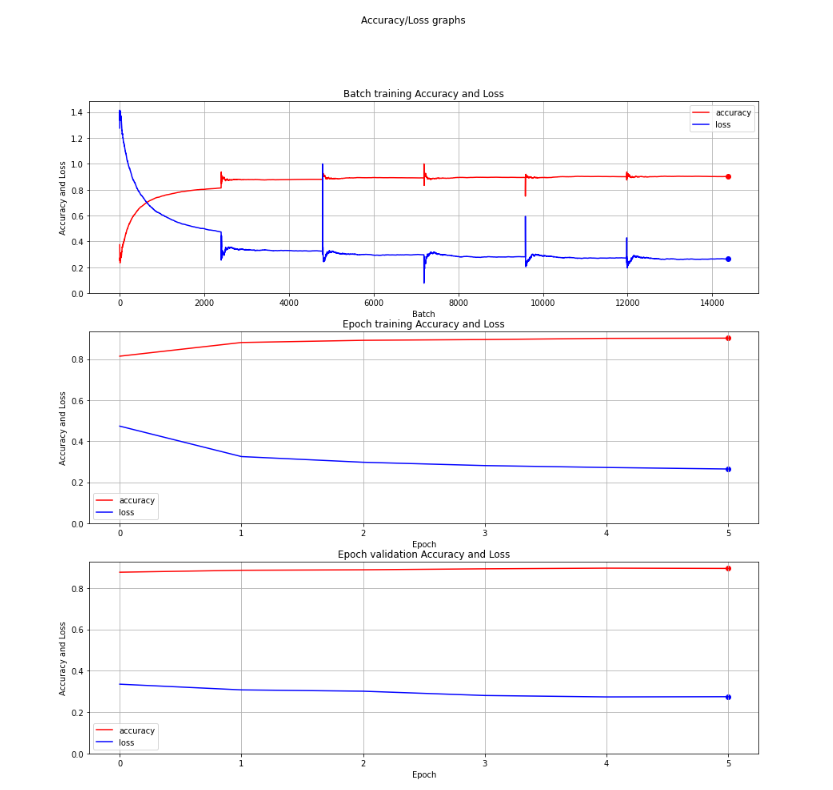
\includegraphics[width=18cm]{head-training}
		\centering
		\caption{График обучения верхних слоёв модели}
	\end{figure}
}

\newcommand{\pictureseven}{
	\begin{figure}[!htbp]
		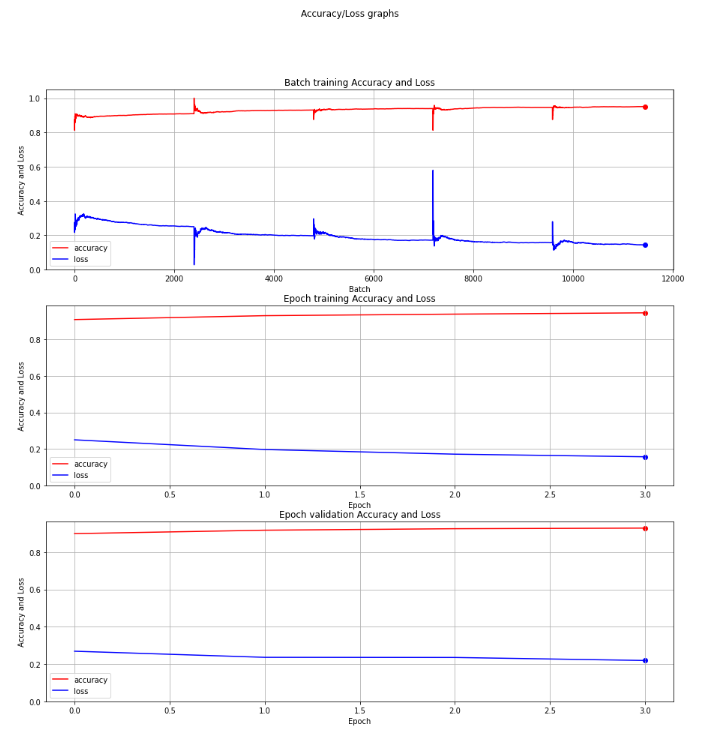
\includegraphics[width=18cm]{full-training}
		\centering
		\caption{График дообучения модели}
	\end{figure}
}